\chapter{Elektromagnetisme Kovarian}\label{ch:b3:covariant-electromagnetism}

Sebuah kawat tembaga mengalirkan arus sepuluh ampere. Elektronnya
menghanyut sepersepuluh milimeter tiap sekon --- lebih lambat daripada
siput --- dan kawat itu netral secara listrik sampai ketelitian yang
menakjubkan. Namun muatan yang bergerak di sampingnya merasakan tarikan
yang terukur. Dilihat dari kerangka muatan itu sendiri, penjelasan
``magnetik''nya menguap: muatannya diam, dan muatan yang diam sama
sekali tidak merasakan gaya magnetik. Yang menariknya, dalam kerangka
itu, adalah medan \emph{listrik} --- yang dipanggil oleh kerelatifan itu
sendiri, karena \omterm{prop:b3:relativistic-kinematics:contraction}{pengerutan panjang} menimbulkan ketakseimbangan sebesar
satu per $10^{24}$ di antara kedua arus muatan dalam kawatnya.
Kemagnetan adalah kelistrikan yang dilihat dari tempat duduk yang
bergerak. Bab ini menuliskan kembali elektromagnetisme jilid Tahun 2
dalam bahasa tiga bab sebelumnya: \omterm{def:b3:covariant-electromagnetism:fourvector}{vektor-empat} untuk muatan dan
potensial, satu tensor antisetangkup yang menyatukan $\vect E$ dan
$\vect B$, serta empat persamaan Maxwell yang mengerut menjadi dua baris
yang berbunyi sama dalam setiap \omterm{thm:b3:relativistic-kinematics:postulates}{kerangka inersial}. Di luar keanggunannya,
hasilnya adalah fisika yang bekerja: bagaimana medan bertransformasi,
mengapa medan muatan yang cepat memipih menjadi cakram, dan mengapa
cahaya elektron relativistik menyapu ke depan bagai lampu sorot ---
yakni asas sumber cahaya sinkrotron yang hari ini menyinari protein dan
baterai dengan sinar-X.

\section{Vektor-empat untuk muatan dan arus}

\begin{definition}[Vektor-empat]\label{def:b3:covariant-electromagnetism:fourvector}
\index{vektor-empat}
Yang disebut \emph{vektor-empat} adalah rangkap empat $a^\mu = (a^0, \vect a)$, $\mu =
0, 1, 2, 3$, yang komponennya bercampur di bawah sebuah dorongan
persis sebagaimana $(ct,
\vect r)$ bercampur:
\[
a'^0 = \gamma(a^0 - \beta a^1) , \qquad
a'^1 = \gamma(a^1 - \beta a^0) , \qquad
a'^{2,3} = a^{2,3}
\]
untuk dorongan sebesar $\beta c$ sepanjang $x$. Sembarang dua
vektor-empat memberikan hasil kali skalar invarian
$a\cdot b = a^0b^0 - \vect a\cdot\vect b$, yakni bilangan yang sama
dalam setiap kerangka --- itulah pola di balik $c^2t^2 - x^2$
dan $E^2 - p^2c^2$. Kedudukan $(ct, \vect r)$ dan \omterm{def:b3:relativistic-dynamics:four-momentum}{momentum-empat}
$(E/c, \vect p)$ adalah dua yang sudah kita miliki; elektromagnetisme
kini memasok tiga lagi: arus, potensial, dan vektor gelombang.
\end{definition}

\begin{proposition}[Arus-empat dan kekekalan muatan]\label{prop:b3:covariant-electromagnetism:fourcurrent}
\index{arus-empat}
Kerapatan muatan $\rho$ dan kerapatan arus $\vect\jmath$ membentuk
arus-empat
\[
J^\mu = (\rho c,\ \vect\jmath\,) :
\]
awan muatan berkerapatan diri $\rho_0$ yang bergerak dengan $\vect u$
mempunyai $J^\mu = \rho_0\gamma_u(c, \vect u)$ --- kerapatannya tumbuh
sebesar $\gamma_u$ karena volume awannya terkerut, sedangkan muatannya
sendiri invarian (sebuah fakta percobaan yang menentukan: atom dengan
elektron dalam yang cepat tetap netral secara tepat). Kekekalan muatan
adalah pernyataan invarian
\[
\frac{\partial(\rho c)}{\partial(ct)} +
\operatorname{div}\vect\jmath = 0 ,
\]
yakni persamaan kesinambungan jilid Tahun 2, yang kini tampak jelas
sebagai hukum yang sama bagi semua pengamat.
\end{proposition}

\begin{proof}[Bukti sebagian]
Awan yang bergerak: sebuah kotak bervolume diri $V_0$ memuat muatan $\rho_0
V_0$; di laboratorium kotaknya terkerut menjadi $V_0/\gamma_u$,
sehingga $\rho =
\gamma_u\rho_0$, dan $\vect\jmath = \rho\vect u$
menurut definisi kerapatan arus. Bahwa $(\rho c, \vect\jmath)$ lalu
bertransformasi sebagai \omterm{def:b3:covariant-electromagnetism:fourvector}{vektor-empat} menyusul karena ia sama dengan
$\rho_0/c$ kali kecepatan-empat $\gamma_u(c, \vect u)$, yang menurut
konstruksinya sudah berupa \omterm{def:b3:covariant-electromagnetism:fourvector}{vektor-empat}. Keinvarianan muatan adalah
masukan percobaan.
\end{proof}

\section{Satu tensor untuk kedua medan}

\begin{definition}[Potensial-empat dan tensor medan]\label{def:b3:covariant-electromagnetism:tensor}
\index{potensial-empat}\index{tensor medan}
Potensial jilid Tahun 2 tersusun menjadi potensial-empat
\[
A^\mu = \Big(\frac{V}{c},\ \vect A\Big) ,
\]
dan medan terukurnya $\vect E = -\vect\nabla V -
\partial_t\vect A$, $\vect B = \operatorname{\vect{curl}}\vect A$
merupakan enam komponen bebas dari satu susunan antisetangkup, yakni
\emph{tensor medan elektromagnetik}
\[
F^{\mu\nu} =
\begin{pmatrix}
0 & -E_x/c & -E_y/c & -E_z/c\\
E_x/c & 0 & -B_z & B_y\\
E_y/c & B_z & 0 & -B_x\\
E_z/c & -B_y & B_x & 0
\end{pmatrix} .
\]
$\vect E$ dan $\vect B$ bukanlah dua medan melainkan enam muka satu
benda; muka mana yang disebut seorang pengamat ``listrik'' bergantung
pada gerak pengamat itu.
\end{definition}

\begin{theorem}[Maxwell, secara kovarian]\label{thm:b3:covariant-electromagnetism:maxwell}
\index{persamaan Maxwell!bentuk kovarian}
Keempat persamaan Maxwell jilid Tahun 2 adalah bentuk komponen dua
pernyataan yang tidak bergantung kerangka: pasangan bersumbernya
(Gauss dan Ampère--Maxwell) adalah
\[
\sum_\mu \partial_\mu F^{\mu\nu} = \mu_0\,J^\nu ,
\]
dan pasangan tanpa sumbernya (tak ada monopol, Faraday) adalah
identitas yang menjamin bahwa $F$ diturunkan dari sebuah
\omterm{def:b3:covariant-electromagnetism:tensor}{potensial-empat}. Gaya Lorentznya adalah $\dd p^\mu/\dd\tau = qF^{\mu\nu}u_\nu$
--- hukum gayanya, termasuk yang magnetik, dalam satu baris. Karena
kedua ruas tiap persamaannya bertransformasi secara serupa,
\emph{teori Maxwell tidak memerlukan koreksi apa pun agar menjadi
relativistik}: ia adalah bagian kerelatifan yang pertama kali selesai,
yang lahir pada 1865.
\end{theorem}

\begin{proof}[Bukti sebagian]
Jabarkanlah komponen $\nu = 0$: $\sum_i\partial_i(E_i/c) =
\mu_0\rho c$, yakni $\operatorname{div}\vect E = \rho/\varepsilon_0$
(dengan memakai $c^2 = 1/\mu_0\varepsilon_0$). Komponen $\nu = 1$
menghimpun $-\partial_t(E_x/c^2) + (\partial_yB_z - \partial_zB_y)
= \mu_0 j_x$: yakni komponen $x$ Ampère--Maxwell. Komponen lainnya
mengulangi pola yang sama; pasangan tanpa sumbernya adalah kesamaan
turunan kedua bersilang $A^\mu$ (yang diperiksa dalam
\cref{exo:b3:covariant-electromagnetism:3}). Bahwa $F^{\mu\nu}$
bertransformasi sebagai tensor (berindeks dua) --- tiap indeksnya
seperti \omterm{def:b3:covariant-electromagnetism:fourvector}{vektor-empat} --- diterima tanpa bukti; akibatnya adalah
proposisi berikutnya.
\end{proof}

\section{Bagaimana medannya bertransformasi}

\begin{proposition}[Transformasi medan]\label{prop:b3:covariant-electromagnetism:transform}
\index{transformasi medan}
Untuk dorongan berkecepatan $\vect v = v\,\vect e_x$: komponen yang
\emph{searah} geraknya tak tersentuh, sedangkan yang melintang bercampur,
\[
E'_x = E_x , \qquad
E'_y = \gamma(E_y - vB_z) , \qquad
E'_z = \gamma(E_z + vB_y) ,
\]
\[
B'_x = B_x , \qquad
B'_y = \gamma\Big(B_y + \frac{v}{c^2}E_z\Big) , \qquad
B'_z = \gamma\Big(B_z - \frac{v}{c^2}E_y\Big) .
\]
Secara ringkas, melintang terhadap dorongannya: $\vect E' = \gamma(\vect E +
\vect v\wedge\vect B)_\perp$ dan $\vect B' = \gamma(\vect B - \vect
v\wedge\vect E/c^2)_\perp$. Medan $\vect B$ murni dalam satu kerangka
menjadi $\vect
E$ dan $\vect B$ dalam kerangka lain: kedua medan itu satu gejala.
\end{proposition}
\admitted

\begin{example}[Kemagnetan dari kawat netral]\label{ex:b3:covariant-electromagnetism:wire}
Sebuah kawat netral mengalirkan arus: kisi positifnya diam, elektronnya
menghanyut. Untuk muatan uji yang bergerak di sampingnya, berpindahlah
ke kerangkanya: kedua arus muatannya terkerut secara \emph{berbeda}
(keduanya berkecepatan berbeda), kawatnya memperoleh muatan garis neto
$\lambda' =
-\gamma vI/c^2$, dan medan listrik radialnya menarik
muatannya dengan gaya yang tepat sama dengan yang disebut laboratorium
$q\vect v\wedge\vect B$. Kemagnetan adalah wujud suku orde kedua
$v u/c^2$ dalam kerelatifan ketika $10^{28}$ muatan dasar tiap meter
bersekongkol: tiap efeknya sangat kecil, tetapi kawatnya netral dengan
ketelitian yang bahkan lebih tinggi, sehingga ketakseimbangan mungil itu
adalah seluruh ceritanya
(\cref{pb:b3:covariant-electromagnetism:1}).
\end{example}

\begin{omfigure}
\begin{tikzpicture}[font=\small, >=Stealth]
  % lab frame
  \begin{scope}
    \draw[thick, fill=omExo!10] (-0.2,0) rectangle (5.4,0.75);
    \foreach \x in {0.3,1.3,2.3,3.3,4.3} \node[omThm] at (\x,0.52) {$\oplus$};
    \foreach \x in {0.8,1.8,2.8,3.8,4.8} {\node[omDef] at (\x,0.22) {$\ominus$};
      \draw[->, omDef] (\x+0.16,0.22) -- (\x+0.42,0.22);}
    \fill[omProp] (2.6,-1.15) circle (2.6pt);
    \draw[->, omProp, thick] (2.75,-1.15) -- (3.55,-1.15);
    \node[anchor=west] at (3.65,-1.15) {$q$, berlaju $v$};
    \draw[->, very thick] (2.6,-0.95) -- (2.6,-0.35);
    \node[anchor=west, font=\footnotesize] at (2.7,-0.62) {$q\vect v\wedge\vect B$};
    \node at (2.6,1.35) {laboratorium: kawat netral, gaya magnetik};
  \end{scope}
  % charge frame
  \begin{scope}[xshift=7.8cm]
    \draw[thick, fill=omExo!10] (-0.2,0) rectangle (5.4,0.75);
    \foreach \x in {0.25,1.15,2.05,2.95,3.85,4.75} {\node[omThm] at (\x,0.52) {$\oplus$};
      \draw[->, omThm] (\x-0.14,0.72) -- (\x-0.4,0.72);}
    \foreach \x in {0.7,1.9,3.1,4.3} \node[omDef] at (\x,0.22) {$\ominus$};
    \fill[omProp] (2.6,-1.15) circle (2.6pt);
    \node[anchor=west] at (2.75,-1.35) {$q$ diam};
    \draw[->, very thick] (2.6,-0.95) -- (2.6,-0.35);
    \node[anchor=west, font=\footnotesize] at (2.7,-0.62) {$q\vect E'$};
    \node at (2.6,1.35) {kerangka muatan: kawat bermuatan, gaya listrik};
  \end{scope}
\end{tikzpicture}

{\small Satu gaya, dua pembukuan. Laboratorium: arus kawat netralnya
membuat $\vect B$, dan muatan yang bergerak merasakan $q\vect v\wedge\vect B$.
Kerangka muatannya: kisi positifnya kini bergerak dan terkerut,
elektronnya (yang di sana lebih lambat) merenggang; kawatnya bermuatan
neto dan $\vect E'$-nyalah yang menarik. Percobaan yang sama, hasil yang
sama.}
\end{omfigure}

\begin{example}[Medan memipih sebuah muatan cepat]\label{ex:b3:covariant-electromagnetism:pancake}
Transformasikanlah medan Coulomb sebuah muatan ke kerangka tempat ia
bergerak pada $\gamma \gg 1$: medan longitudinalnya tak berubah
sedangkan yang melintang dikalikan $\gamma$. Medan yang tadinya bulat
memipih menjadi cakram bersudut bukaan $\sim 1/\gamma$ di sekitar bidang
yang melalui muatannya --- disertai, melintang terhadap geraknya, sebuah
cincin magnetik $B' = vE'/c^2$. Bagi pengamat yang diam, lewatnya proton
LHC ($\gamma \approx 7000$) adalah tamparan $\vect E$ dan $\vect B$
yang nyaris bersilangan selama kurang dari satu pikosekon: hampir sebuah
pulsa cahaya --- itulah sebabnya berkas cepat berbicara kepada materi
sebagaimana foton berbicara.
\end{example}

\begin{omfigure}
\begin{tikzpicture}[font=\small, >=Stealth]
  % static charge
  \begin{scope}
    \fill[omThm] (0,0) circle (2.6pt);
    \foreach \a in {0,30,...,330} \draw[->, omDef] (\a:0.25) -- (\a:1.75);
    \node at (0,-2.5) {dalam keadaan diam: medan Coulomb isotropik};
  \end{scope}
  % moving charge
  \begin{scope}[xshift=8.0cm]
    \fill[omThm] (0,0) circle (2.6pt);
    \draw[->, very thick] (0.3,-2.1) -- (1.5,-2.1) node[right] {$v \approx c$};
    \foreach \a/\l in {90/1.95, 75/1.5, 105/1.5, 60/0.85, 120/0.85,
                       270/1.95, 255/1.5, 285/1.5, 240/0.85, 300/0.85,
                       0/0.35, 180/0.35, 30/0.45, 150/0.45, 210/0.45, 330/0.45}
      \draw[->, omDef] (\a:0.25) -- (\a:\l);
    \node at (0,-2.5) {};
    \node at (0.3,-2.65) {};
    \node at (0,-2.9) {};
  \end{scope}
  \node at (8.0,-2.5) {bergerak: medannya memipih menjadi $\sim 1/\gamma$};
\end{tikzpicture}

{\small Medan listrik sebuah muatan titik, dalam keadaan diam dan pada
laju tinggi: dorongannya mengalikan komponen melintangnya dengan
$\gamma$ dan membiarkan komponen longitudinalnya, sehingga medannya
terperas menjadi cakram yang tegak lurus terhadap geraknya.}
\end{omfigure}

\section{Invarian, cahaya, dan efek lampu sorot}

\begin{proposition}[Kedua invarian medan]\label{prop:b3:covariant-electromagnetism:invariants}
\index{invarian medan}
Dari $F^{\mu\nu}$ hanya dapat dibangun tepat dua skalar bebas:
\[
E^2 - c^2B^2
\qquad\text{dan}\qquad
\vect E\cdot\vect B ,
\]
yang sama dalam setiap \omterm{thm:b3:relativistic-kinematics:postulates}{kerangka inersial}. Akibatnya: jika $E > cB$ di
suatu tempat (dengan $\vect E\cdot\vect B = 0$), ada kerangka yang
melihat medan listrik murni di sana; jika $E < cB$, ada kerangka yang
melihatnya magnetik murni; dan gelombang cahaya bidang, dengan $E = cB$
dan $\vect E\perp\vect B$, mempunyai \emph{kedua} invariannya nol ---
ia tetap cahaya dalam setiap kerangka: tak ada dorongan yang dapat
mengubahnya menjadi medan statis, hanya menggesernya ke merah. Kita
tidak dapat menyusul gelombang cahaya; pertanyaan Einstein semasa remaja
terjawab sendiri lewat dua invarian.
\end{proposition}

\begin{proof}[Bukti sebagian]
Periksalah keinvariannya di bawah dorongan bakunya dengan penyulihan
langsung
\cref{prop:b3:covariant-electromagnetism:transform}
(\cref{exo:b3:covariant-electromagnetism:6}); bahwa tak ada invarian
bebas ketiga diterima tanpa bukti. Untuk gelombangnya: $E = cB$ dan
keortogonalannya membuat keduanya nol; kerangka dengan medan statis
akan menuntut invarian yang tak nol.
\end{proof}

\begin{proposition}[Vektor gelombang-empat, Doppler dan aberasi]\label{prop:b3:covariant-electromagnetism:wavevector}
\index{aberasi}\index{efek lampu sorot}
Frekuensi dan arah gelombang bidang membentuk \omterm{def:b3:covariant-electromagnetism:fourvector}{vektor-empat} null
$k^\mu = (\omega/c, \vect k)$, $\|\vect k\| = \omega/c$.
Mentransformasikannya langsung memberikan rumus Doppler relativistik
\cref{ch:b3:relativistic-kinematics} sekaligus \emph{aberasi}
arahnya:
\[
\cos\theta' = \frac{\cos\theta - \beta}{1 - \beta\cos\theta} .
\]
Dibaca terbalik, sumber yang memancar isotropik dalam kerangka diamnya
memancarkan, di laboratorium, separuh cahayanya ke dalam kerucut depan $\theta
\lesssim 1/\gamma$: itulah \emph{\omterm{prop:b3:covariant-electromagnetism:wavevector}{efek lampu sorot}}. Elektron
yang beredar pada $\gamma \sim 10^4$ dalam cincin penyimpan menyapukan
lampu sorot sinar-X selebar $\qty{0.1}{mrad}$ mengelilingi cincinnya ---
yakni cahaya sinkrotron yang mengisi jalur berkas kristalografi protein.
\end{proposition}

\begin{proof}[Bukti sebagian]
Fasenya $\omega t - \vect k\cdot\vect r = k^\mu x_\mu$ menghitung
puncak gelombang yang melewati peristiwa --- sebuah invarian ---
sehingga $k^\mu$ harus bertransformasi sebagai \omterm{def:b3:covariant-electromagnetism:fourvector}{vektor-empat}.
Kenakanlah dorongannya pada $(\omega/c, k\cos\theta,
k\sin\theta, 0)$: komponen waktunya memberikan Doppler, dan nisbah
komponen ruangnya memberikan rumus aberasinya. Dengan mengambil
$\theta' =
90^\circ$ (sinar menyamping dalam kerangka sumbernya): $\cos\theta =
\beta$, yakni $\theta \approx 1/\gamma$ untuk
$\gamma \gg 1$ --- separuh bolanya terlipat ke dalam kerucut depan.
\end{proof}

\begin{omfigure}
\begin{tikzpicture}[font=\small, >=Stealth]
  % isotropic source
  \begin{scope}
    \fill[omThm] (0,0) circle (2.4pt);
    \foreach \a in {0,45,...,315} \draw[->, omExo] (\a:0.3) -- (\a:1.5);
    \node at (0,-2.2) {kerangka diam: isotropik};
  \end{scope}
  % beamed
  \begin{scope}[xshift=7.6cm]
    \fill[omThm] (0,0) circle (2.4pt);
    \draw[->, thick] (-1.9,0) -- (-0.6,0);
    \node at (-2.35,0) {$v$};
    \draw[->, omExo] (0.3,0.06) -- (2.6,0.55);
    \draw[->, omExo] (0.3,-0.06) -- (2.6,-0.55);
    \draw[->, omExo, very thick] (0.3,0) -- (2.9,0);
    \draw[->, omExo] (0.25,0.16) -- (1.5,1.0);
    \draw[->, omExo] (0.25,-0.16) -- (1.5,-1.0);
    \draw[->, omExo] (-0.1,0.28) -- (-0.5,1.0);
    \draw[->, omExo] (-0.1,-0.28) -- (-0.5,-1.0);
    \draw[dashed] (0,0) -- (3.1,0.85);
    \draw[dashed] (0,0) -- (3.1,-0.85);
    \node[anchor=west, font=\footnotesize] at (3.0,0.5) {$\sim 1/\gamma$};
    \node at (0.9,-2.2) {laboratorium: lampu sorot ke depan};
  \end{scope}
\end{tikzpicture}

{\small Aberasi melipat radiasi sumber yang cepat ke dalam kerucut depan
bersetengah sudut $\sim 1/\gamma$: itulah \omterm{prop:b3:covariant-electromagnetism:wavevector}{efek lampu sorot}, sekaligus
asas kerja sumber cahaya sinkrotron.}
\end{omfigure}

\begin{method}[Bekerja secara kovarian]\label{met:b3:covariant-electromagnetism:method}
(1) Kenalilah \omterm{def:b3:covariant-electromagnetism:fourvector}{vektor-empat} yang berperan ($x^\mu$, $P^\mu$, $J^\mu$,
$A^\mu$, $k^\mu$) lalu utamakanlah hasil kali invariannya daripada
komponennya. (2) Untuk mentransformasikan medan, pisahkanlah menjadi
komponen searah dan melintang terhadap dorongannya lalu kenakanlah
\cref{prop:b3:covariant-electromagnetism:transform}. (3) Periksalah
kedua invariannya sebelum dan sesudahnya --- itulah pendeteksi galat
tercepat dalam pokok bahasan ini. (4) Ketika soal magnetik tampak
membingungkan, menumpanglah bersama muatannya: dalam kerangkanya hanya
$\vect E'$ yang bekerja. (5) Percayailah Maxwell: persamaannya tak
pernah memerlukan ``koreksi'' relativistik, hanya pembacaan relativistik.
\end{method}

\begin{omfigure}
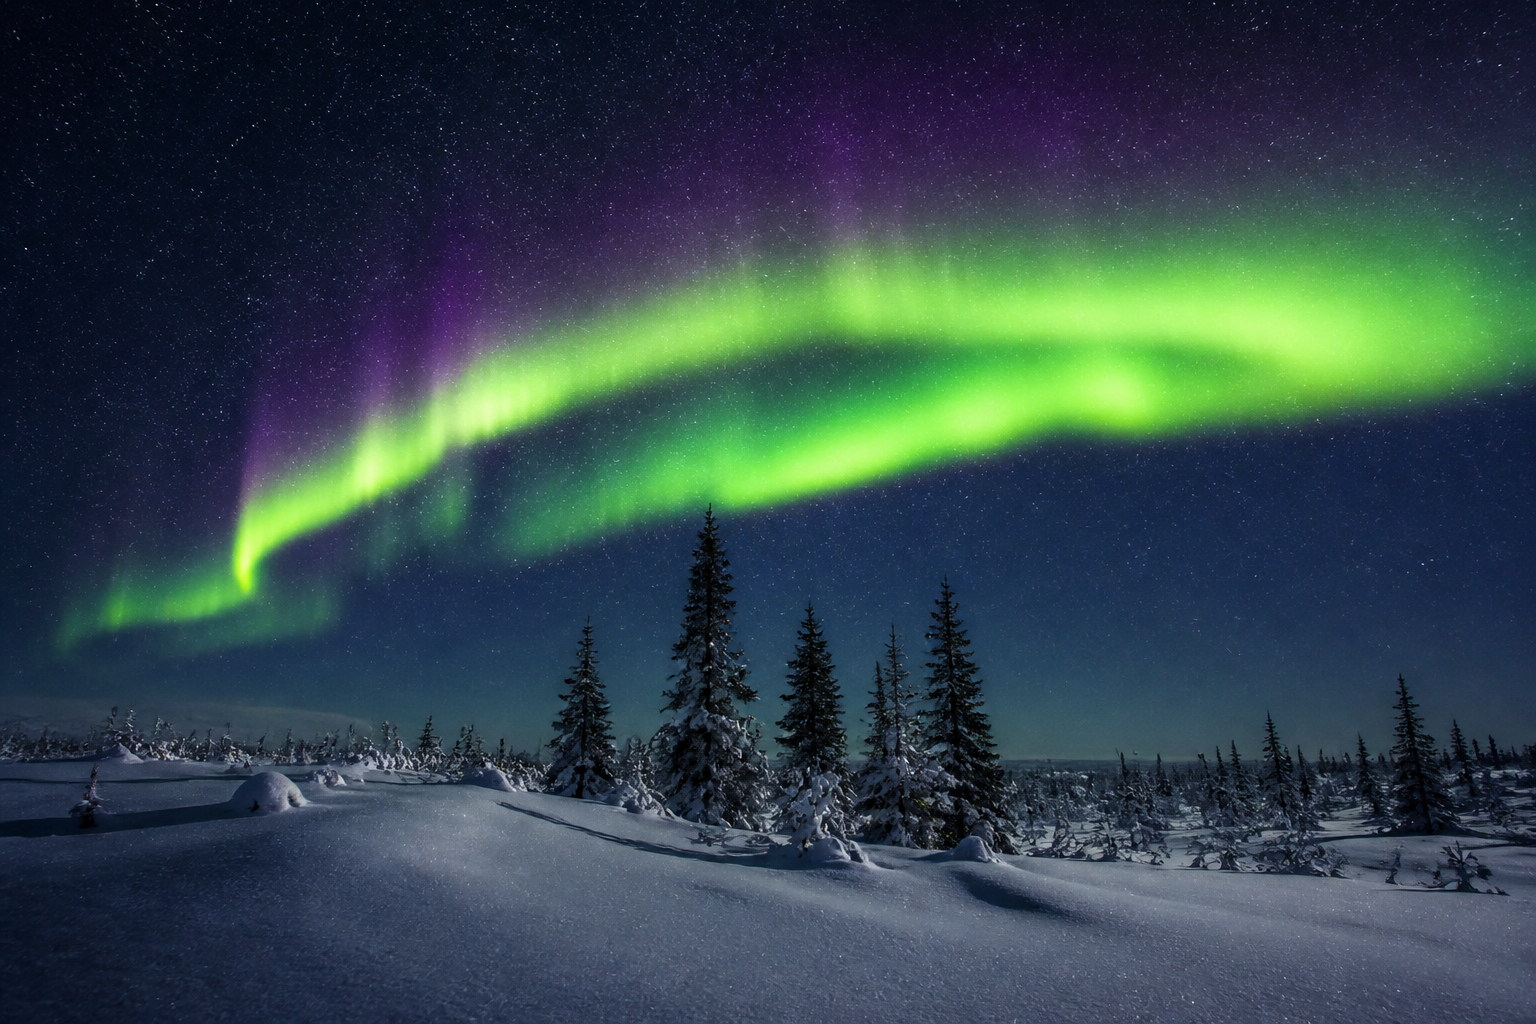
\includegraphics[width=0.58\linewidth]{images/book5/ai/b5-24-aurora-arc.png}

{\small Aurora: muatan angin surya yang dikemudikan medan magnet Bumi ke dalam atmosfer kutub. Apa yang disebut seorang pengamat sebagai kemudi magnetik, disebut pengamat lain sebagai percepatan listrik --- medannya bercampur di bawah transformasi bab ini.}
\end{omfigure}

\section{Latihan}

\begin{exercise}[$\star$]\label{exo:b3:covariant-electromagnetism:1}
(a) Doronglah $a^\mu = (5, 3, 0, 0)$ (dalam satuan $a_0$ tertentu)
sebesar $\beta =
0.6$: hitunglah $a'^\mu$ lalu periksalah bahwa
$a\cdot a$ tak berubah. (b) Tunjukkanlah bahwa jumlah dua \omterm{def:b3:covariant-electromagnetism:fourvector}{vektor-empat}
adalah \omterm{def:b3:covariant-electromagnetism:fourvector}{vektor-empat}. (c) Apakah $(c,
\vect v)$ sebuah partikel merupakan \omterm{def:b3:covariant-electromagnetism:fourvector}{vektor-empat}? Dan $\gamma(c, \vect v)$? (d)
Mengapa ``medan listrik'' saja bukan bagian \omterm{def:b3:covariant-electromagnetism:fourvector}{vektor-empat} mana pun?
\end{exercise}

\begin{exercise}[$\star$]\label{exo:b3:covariant-electromagnetism:2}
Kawat tembaga berpenampang \qty{1.0}{mm^2} mengalirkan \qty{10}{A};
kerapatan elektron hantarannya $n = \qty{8.5e28}{m^{-3}}$. (a)
Hitunglah laju hanyutnya. (b) Tuliskanlah $J^\mu$ untuk fluida
elektronnya dan untuk kisinya. (c) Periksalah persamaan
kesinambungannya untuk masing-masing. (d) Kawatnya netral: berapa
$J^\mu$ untuk kawat seluruhnya, dan komponen mana yang bertahan?
\end{exercise}

\begin{exercise}[$\star$]\label{exo:b3:covariant-electromagnetism:3}
(a) Dari matriks $F^{\mu\nu}$, bacalah komponen mana yang memberikan
$E_y$ dan $B_x$. (b) Tuliskanlah $F^{\mu\nu}$ untuk medan seragam murni
$\vect B = B\vect e_z$, dan untuk medan gelombang bidang
($\vect E = E\vect e_y$, $\vect B = (E/c)\vect e_z$). (c) Periksalah
pada komponennya bahwa $F^{\mu\nu} = \partial^\mu A^\nu - \partial^\nu
A^\mu$ menghasilkan kembali $\vect B = \operatorname{\vect{curl}}\vect A$ untuk
$\mu\nu = 12$. (d) Mengapa $F$ harus antisetangkup agar gaya
$qF^{\mu\nu}u_\nu$ tidak melakukan usaha dalam kerangka partikelnya sendiri?
\end{exercise}

\begin{exercise}[$\star$]\label{exo:b3:covariant-electromagnetism:4}
Sebuah kapasitor pelat sejajar yang diam menyimpan $\vect E = E_0\vect e_y$,
tanpa $\vect B$. Berikanlah $\vect E'$ dan $\vect B'$ dalam kerangka
yang bergerak (a) sepanjang $\vect e_y$ (tegak lurus pelatnya); (b)
sepanjang $\vect
e_x$ (sejajar pelatnya), lalu tafsirkanlah $\vect B'$
yang muncul sebagai medan muatan permukaan yang bergerak; (c)
periksalah invariannya pada kasus (b); (d) pada kasus (b), pelatnya juga
terkerut: besaran mana ($\sigma$? $E'$? jarak antarpelatnya?) yang
berubah, dan selaras dengan apa?
\end{exercise}

\begin{exercise}[$\star\star$]\label{exo:b3:covariant-electromagnetism:5}
Ggl gerak yang disatukan. Sebuah batang penghantar meluncur dengan
$\vect v$ pada rel melintasi $\vect B$ yang seragam. (a) Pembukuan
laboratorium: gaya mana yang menggerakkan elektronnya sepanjang
batangnya, dan berapa ggl yang dihasilkannya? (b) Pembukuan kerangka
batangnya: medan apa yang menggerakkannya, dan dari mana ia datang
dalam \cref{prop:b3:covariant-electromagnetism:transform}? (c)
Tunjukkanlah bahwa kedua ggl itu sesuai pada orde $v/c$. (d) Aturan
fluks Faraday jilid Tahun 1 mencakup kasus ``rangkaian bergerak'' dan
``medan berubah'' dengan satu rumus: apa kata kerelatifan tentang
mengapa penyatuan itu memang harus bekerja?
\end{exercise}

\begin{exercise}[$\star\star$]\label{exo:b3:covariant-electromagnetism:6}
(a) Dengan memakai \cref{prop:b3:covariant-electromagnetism:transform},
periksalah lewat perhitungan langsung bahwa
$E'^2 - c^2B'^2 = E^2 - c^2B^2$ untuk dorongan sepanjang $x$. (b)
Periksalah $\vect E'\cdot\vect B' = \vect
E\cdot\vect B$. (c) Sebuah daerah memuat $\vect E$ dan $\vect B$ yang
tegak lurus dengan $E = 2cB$: carilah kerangka dengan medan listrik
murni (arah dan lajunya). (d) Mengapa tak ada kerangka yang dapat
membuat medan gelombang cahaya bidang menjadi listrik murni atau
magnetik murni?
\end{exercise}

\begin{exercise}[$\star\star$]\label{exo:b3:covariant-electromagnetism:7}
Medan bersilang. Di laboratorium, $\vect E = E\vect e_y$ dan $\vect B =
B\vect e_z$ dengan $E < cB$. (a) Tunjukkanlah bahwa kerangka yang
bergerak pada $\vect v_{\text{d}} = (E/B)\,\vect e_x$ melihat medan
magnetik murni. (b) Perikanlah gerak muatan yang dilepaskan dalam
keadaan diam, dilihat dari kerangka itu dan kembali di laboratorium
(sikloid yang menghanyut pada $v_{\text{d}}$). (c)
Penapis kecepatan jilid Tahun 1 meloloskan partikel berlaju $E/B$ tanpa
pembelokan: turunkanlah kembali hal itu dalam satu baris dari (a). (d)
Apa yang terjadi, secara kualitatif, ketika $E > cB$ --- dan mengapa
muslihat kerangka hanyutnya lalu menjadi mustahil?
\end{exercise}

\begin{exercise}[$\star\star$]\label{exo:b3:covariant-electromagnetism:8}
Vektor gelombang-empat $k^\mu = (\omega/c, \vect k)$. (a) Tunjukkanlah
bahwa menuntut fasenya invarian memaksa $k^\mu$ bertransformasi sebagai
\omterm{def:b3:covariant-electromagnetism:fourvector}{vektor-empat}. (b) Turunkanlah rumus Doppler longitudinalnya dari
komponen waktunya. (c) Turunkanlah rumus aberasinya. (d) Aberasi cahaya
bintang: Bumi mengorbit pada \qty{29.8}{km/s}; melalui sudut berapa
kedudukan semu sebuah bintang menyapu sepanjang setahun? (Bradley
mengukur $20.5''$ pada 1728 --- bukti langsung pertama bahwa Bumi bergerak.)
\end{exercise}

\begin{exercise}[$\star\star$]\label{exo:b3:covariant-electromagnetism:9}
Sebuah muatan $q$ bergerak dengan $\vect v = v\vect e_x$ tetap, $\gamma \gg
1$. (a) Dengan mentransformasikan medan Coulombnya, tunjukkanlah bahwa
pada bidang melintang yang melalui muatannya medannya terdorong menjadi
$\gamma
q/4\pi\varepsilon_0b^2$ pada jarak $b$, sedangkan tepat di depan dan di
belakangnya ia terhimpit sebesar $1/\gamma^2$. (b) Tunjukkanlah bahwa
pengamat diam pada jarak $b$ melihat pulsa medan berdurasi
$\sim b/\gamma v$. (c) Untuk proton LHC yang lewat pada $b = \qty{1}{cm}$:
berapa medan puncaknya dan durasi pulsanya? (d) Dalam pengertian apa
tepatnya pulsa ini ``hampir cahaya''? (Periksalah $E' \approx cB'$ dan
invariannya.)
\end{exercise}

\begin{exercise}[$\star\star\star$]\label{exo:b3:covariant-electromagnetism:10}
Mengejar gelombang cahaya. Sebuah gelombang bidang mempunyai $\vect E = E_0\vect e_y
\cos(\omega(t - x/c))$, $\vect B = (E_0/c)\vect e_z\cos(\omega(t -
x/c))$. Seorang pengamat mengejarnya pada $\beta$. (a)
Transformasikanlah medannya: tunjukkanlah
$E'_0 = E_0\sqrt{(1-\beta)/(1+\beta)}$ dan $B'_0 = E'_0/c$. (b)
Tunjukkanlah bahwa frekuensinya bertransformasi dengan faktor yang
sama: gelombangnya tetap gelombang, tergeser merah, dengan $E' = cB'$
selalu. (c) Apa yang terjadi pada kerapatan energi gelombangnya
(sebanding dengan $E^2$) dan pada cacah fotonnya? (d) Simpulkanlah: apa
yang dituntut oleh ``menumpang di samping berkas cahaya'', dan invarian
mana yang melarangnya?
\end{exercise}

\begin{exercise}[$\star\star\star$]\label{exo:b3:covariant-electromagnetism:11}
Cahaya sinkrotron dan matinya mesin elektron melingkar. Sebuah muatan
ultrarelativistik pada lingkaran berjejari $r$ memancarkan daya
$P = q^2c\gamma^4/6\pi\varepsilon_0r^2$ (diterima tanpa bukti --- rumus
Larmor jilid Tahun 2, yang didorong). (a) Tunjukkanlah bahwa energi yang
hilang tiap putaran adalah $\Delta E = q^2\gamma^4/3\varepsilon_0r$. (b) LEP:
elektron pada \qty{100}{GeV} dengan $r = \qty{3.1}{km}$: hitunglah $\gamma$ dan
$\Delta E$ tiap putaran --- berapa bagian energi berkasnya yang harus
dibeli ulang tiap putaran? (c) LHC: proton pada \qty{6.8}{TeV}, dalam
terowongan yang sama: hitunglah $\Delta E$ tiap putaran lalu
bandingkanlah. (d) Jelaskanlah, dengan faktor $\gamma^4 =
(E/mc^2)^4$, mengapa penerus mesin elektron itu berupa penumbuk
\emph{linear} atau cincin yang jauh lebih besar, dan mengapa cincin
proton bertahan.
\end{exercise}

\begin{exercise}[$\star\star\star$]\label{exo:b3:covariant-electromagnetism:12}
Siklotron relativistik. Sebuah muatan dalam $\vect B$ yang seragam, pada
laju relativistik. (a) Dari $\dd\vect p/\dd t = q\vect v\wedge\vect
B$ dengan $E$ tetap, tunjukkanlah bahwa orbitnya berupa lingkaran yang
ditempuh pada $\omega = qB/\gamma m$: frekuensi siklotronnya turun
seiring energinya.
(b) Siklotron klasik mendorong pada $\omega_0 = qB/m$ yang tetap:
tunjukkanlah bahwa setelah $N$ putaran dengan $\gamma - 1$ tumbuh secara
linear sampai nilai akhirnya $\Gamma$, selisih fase yang terkumpul
mencapai seperempat periode RF ketika $\Gamma \approx 1/2N$; untuk
$N = 100$ putaran, energi kinetik proton sebesar apakah itu, dan
bagaimana perbandingannya dengan langit-langit sejarah siklotron klasik
(sekitar \qty{20}{MeV}, yang dibeli dengan kelonggaran dan tegangan
tambahan)? (c) Ada dua
penawarnya: menaikkan frekuensinya (sinkrosiklotron) atau membentuk
$B(r)$ agar tumbuh seperti $\gamma$ (siklotron isokron): jelaskanlah
masing-masing dalam satu kalimat. (d) Siklotron isokron PSI
menghasilkan proton \qty{590}{MeV}: sebesar faktor berapa medannya di
tepi melebihi medan pusatnya?
\end{exercise}

\section{Soal: Kemagnetan pada kecepatan siput}

\begin{problem}[{Soal akhir pekan --- bagaimana ketakseimbangan
$10^{-24}$ menjalankan tiap motor}]\label{pb:b3:covariant-electromagnetism:1}
Elektron menghanyut melalui kabel lampu lebih lambat daripada madu
merambat, dan $v^2/c^2$ bagi hanyutan itu bernilai $10^{-24}$ --- namun
gaya magnetik yang dihasilkannya mengangkat mobil di tempat rongsokan.
Soal ini melakukan pembukuan dua kerangka selengkapnya untuk kawat lurus
dan muatan yang bergerak, lalu menemukan kerelatifan bersembunyi dalam
tiap elektromagnet. Data: kawat tembaga, penampang $S = \qty{1.0}{mm^2}$,
arus $I = \qty{10}{A}$, kerapatan elektron hantaran
$n = \qty{8.5e28}{m^{-3}}$; muatan uji
$q = \qty{1}{\micro C}$ pada jarak $d = \qty{1.0}{cm}$, yang bergerak
sejajar kawatnya pada $v = \qty{e5}{m/s}$ (laju berkas ion, agar
bilangannya tetap terlihat); $\mu_0 = 4\pi\times10^{-7}\,\unit{H/m}$.

\medskip\noindent\textbf{Bagian I --- Pembukuan kerangka laboratorium.}
\begin{enumerate}
  \item Hitunglah laju hanyut elektronnya $u$, beserta $u^2/c^2$.
  \item Modelkanlah kawatnya sebagai dua muatan garis yang bertumpang
        tindih: kisi $+\lambda$ yang diam dan elektron $-\lambda$ yang
        menghanyut pada $u$, dengan $I = \lambda u$. Hitunglah $\lambda$.
  \item Hitunglah $B$ pada kedudukan muatannya dan gaya magnetik
        $F = qvB$ padanya --- termasuk arahnya, untuk $v$ yang sejajar
        arus konvensional $I$ (ingatlah: arus sejajar saling menarik).
  \item Mengapa tak ada gaya \emph{listrik} di laboratorium?
  \item Berapa medan listrik kawat yang sama jika ia membawa muatan
        neto sebesar satu elektron berlebih tiap meter: bandingkanlah
        gaya yang akan dikerahkannya pada $q$ dengan gaya magnetik pada
        pertanyaan 3, lalu simpulkanlah seberapa teliti ``netral'' harus
        diukur sebelum kemagnetan boleh dinisbahkan.
  \item Muatan \qty{1}{\micro C} pada \qty{e5}{m/s}: apakah gaya pada
        pertanyaan 3 terukur? (Bandingkanlah dengan berat sebutir pasir,
        $\sim\qty{e-6}{N}$.)
\end{enumerate}

\medskip\noindent\textbf{Bagian II --- Berpindah tempat duduk.}
Berpindahlah ke kerangka muatan ujinya (berlaju $v$ sepanjang kawatnya).
\begin{enumerate}[resume]
  \item Dalam kerangka itu, berapa kecepatan kisinya dan kecepatan
        elektronnya (yang menghanyut berlawanan dengan $I$, sehingga
        bertambah laju pada dorongan ini --- gabungkanlah dengan benar)?
  \item Diintegralkan pada penampang kawatnya, arus-empat tiap satuan
        panjangnya adalah $(c\lambda_{\text{tot}}, I, 0, 0)$ dengan
        $\lambda_{\text{tot}} = 0$ di sini. Transformasikanlah lalu
        tunjukkanlah bahwa muatan garis kawatnya dalam kerangka barunya
        adalah
        \[
        \lambda' = -\gamma_v\,\frac{vI}{c^2} .
        \]
  \item Hitunglah $\lambda'$, dalam coulomb tiap meter dan dalam muatan
        elektron tiap meter. Arus yang mana yang menjadi lebih rapat, dan
        mengapa (kerutkanlah tiap arusnya sendiri-sendiri jika Anda mau)?
  \item Hitunglah medan listrik $E' = \lambda'/2\pi\varepsilon_0d$
        pada muatannya, beserta gaya listrik $qE'$ padanya.
  \item Bandingkanlah $qE'$ dengan $qvB$ laboratorium pada Bagian I,
        lalu jelaskanlah faktor sisa $\gamma_v \approx 1 + \num{5.6e-8}$
        (hukum transformasi \omterm{def:b3:covariant-electromagnetism:fourvector}{vektor-empat} manakah yang mengaitkan kedua
        gayanya?).
  \item Dalam kerangka ini ada pula medan magnet (kawatnya tetap
        mengalirkan arus): mengapa medan itu tidak mengerahkan gaya di
        sini?
\end{enumerate}

\medskip\noindent\textbf{Bagian III --- Pelajaran dari bilangannya.}
\begin{enumerate}[resume]
  \item Ketakseimbangan nisbinya $|\lambda'|/\lambda$: hitunglah lalu
        tuliskanlah sebagai $\gamma_v vu/c^2$.
  \item Bagaimana efek berorde $10^{-19}$ dari muatan kawatnya dapat
        menghasilkan gaya makroskopis? (Bilangan raksasa apa yang
        dikalikannya?)
  \item Dua kawat sejajar yang masing-masing mengalirkan \qty{10}{A}
        pada jarak \qty{1}{cm}: hitunglah gaya tiap meternya, lalu
        periksalah terhadap nilai bermutu definisi
        $2 \times 10^{-7}\,I_1I_2/d$ newton tiap meter.
  \item Sebuah elektromagnet adalah sepuluh ribu lilitan cerita ini:
        perkirakanlah medan kumparan berlilitan \qty{e4}{} tiap meter
        yang mengalirkan \qty{10}{A} (rumus solenoida jilid Tahun 1),
        beserta gaya tiap sentimeter persegi yang dikerahkannya pada
        besi ($\sim B^2/2\mu_0$).
  \item Seandainya kerelatifan dimatikan ($c \to \infty$ dalam
        transformasinya), apa yang akan tersisa dari $\lambda'$, dari
        gaya $B$, dari motor dan magnet tempat rongsokan?
  \item Mengapa muatan uji yang \emph{diam} di dekat kawatnya tidak
        merasakan apa pun, walaupun elektronnya mengalir melewatinya?
        (Peniadaan yang mana yang melindunginya, dan sampai ketelitian
        berapa?)
\end{enumerate}

\medskip\noindent\textbf{Bagian IV --- Melampaui kawatnya.}
\begin{enumerate}[resume]
  \item Jilid Tahun 2 menurunkan medan magnet dari hukum Ampère
        dengan arus sebagai sumber yang diberikan. Apa yang ditambahkan
        bab ini pada pembukuan itu --- \emph{apakah} medan magnet itu,
        dilihat dari soal ini?
  \item Magnet besi tidak mempunyai baterai: apa yang berperan sebagai
        arus dalam kemagnetan tetap (satu kalimat; jawaban mikroskopis
        yang jujur bersifat kuantum dan menunggu lima bab lagi)?
  \item Sebuah berkas elektron tunggal dalam vakum (tanpa kisi):
        apakah pengamat yang ikut bergerak melihatnya menarik atau
        menolak dirinya sendiri lebih kuat daripada yang dilihat
        pengamat laboratorium? Damaikanlah pembukuan kedua kerangka
        tentang pencekikan diri sebuah berkas.
  \item Buatlah butir terakhir itu kuantitatif: tunjukkanlah bahwa dua
        berkas sejajar bermuatan sejenis yang bergerak bersama pada
        $\beta$ saling menolak dengan gaya neto (tolakan listrik
        dikurangi tarikan magnetik) yang berkurang tepat sebesar
        $1/\gamma^2$ dari nilai diamnya --- lalu katakanlah pembukuan
        kerangka mana yang membuat faktor itu gamblang.
  \item Energi untuk sebuah lampu tiba dengan laju hampir $c$ sedangkan
        elektronnya menghanyut satu meter tiap jam: apa yang
        sesungguhnya membawa energi sepanjang kabelnya (ingatlah vektor
        Poynting jilid Tahun 2)?
  \item Perkirakanlah $vu/c^2$ untuk elektron pada soal ini dan muatan
        uji seorang pejalan kaki ($v = \qty{1}{m/s}$): bahkan di sana,
        gayanya terukur pada orde pertama dengan jarum kompas ---
        siapakah yang memperagakan arus membelokkan kompas, dan pada
        tahun berapa?
  \item Ringkaslah hasil bernama itu: kawat netral \qty{10}{A}, yang
        dipandang dari tempat duduk yang bergerak pada \qty{e5}{m/s},
        membawa muatan relativistik $-\qty{e-11}{C/m}$ --- dan galat
        pembukuan berorde $10^{-24}$ dari \omterm{prop:b3:relativistic-kinematics:contraction}{pengerutan panjang} itu,
        dikalikan $10^{28}$ elektron, adalah seluruh gaya magnetik di
        laboratorium.
\end{enumerate}
\end{problem}
